% Lists frame
\section{GPC}
\begin{frame}{Wielowymiarowy GPC}
Projekt pętli regulacji z zastosowaniem wielowymiarwego algorytmu GPC:
\begin{itemize}
    \item Wyznaczenie wielowymiarowej odpowiedzi impulsowej
    \item Model w postacji odpowiedzi skokowej
    \item Rozwiązanie problemu optymalizacji
    \item Wyznaczenie wektora optymalnych przyrostów sterowań
\end{itemize}
Wszystkie sygnały sterujące wpływają na sygnały wyjściowe. 
\end{frame}

\begin{frame}{Wielowymiarowy GPC}
Wyznaczenie wielowymiarowej odpowiedzi impulsowej:
	\begin{center}
		\begin{figure}[H]
            		
\includegraphics[scale=0.7]{images/odp_GPC.png}
		\end{figure}
	\end{center}
\end{frame}

\begin{frame}{Wielowymiarowy GPC}
Model w postacji odpowiedzi skokowej:
	\begin{center}
		\begin{figure}[H]
            		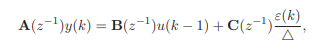
\includegraphics[scale=0.7]{images/model_GPC.png}
		\end{figure}
	\end{center}
gdzie A, B i C są macierzami wielomianowymi
\begin{center}
		\begin{figure}[H]
            		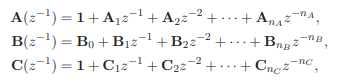
\includegraphics[scale=0.7]{images/macierze_GPC.png}
		\end{figure}
	\end{center}
\end{frame}

\begin{frame}{Wielowymiarowy GPC}
Model w przypadku działania szumów białych:
	\begin{center}
		\begin{figure}[H]
            		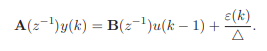
\includegraphics[scale=0.9]{images/postac_GPC.png}
		\end{figure}
	\end{center}
\end{frame}

\begin{frame}{Wielowymiarowy GPC}
Rozwiązanie problemu optymalizacji:
	\begin{center}
		\begin{figure}[H]
            		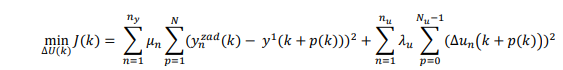
\includegraphics[scale=0.6]{images/cel_DMC.png}
		\end{figure}
	\end{center}
Zastosowanie terjektorii referencyjnej w miejsce trajektorii wartości zadanych
	\begin{center}
		\begin{figure}[H]
            		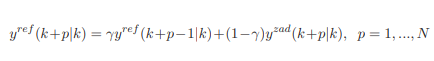
\includegraphics[scale=0.65]{images/referencyjna_GPC.png}
		\end{figure}
	\end{center}
\end{frame}


\begin{frame}{Wielowymiarowy GPC}
Określenie pętli regulacji:
	\begin{center}
		\begin{figure}[H]
            		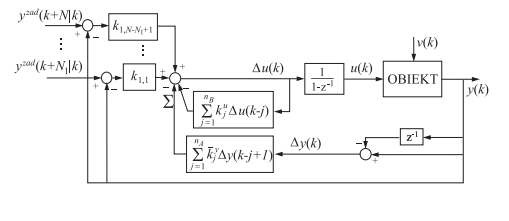
\includegraphics[scale=0.7]{images/SISOGPC.png}
          			 \caption{Schemat układu regulacji}
		\end{figure}
	\end{center}
\end{frame}

\begin{frame}{Wielowymiarowy GPC}
Wyniki działania:
	\begin{center}
		\begin{figure}[H]
            		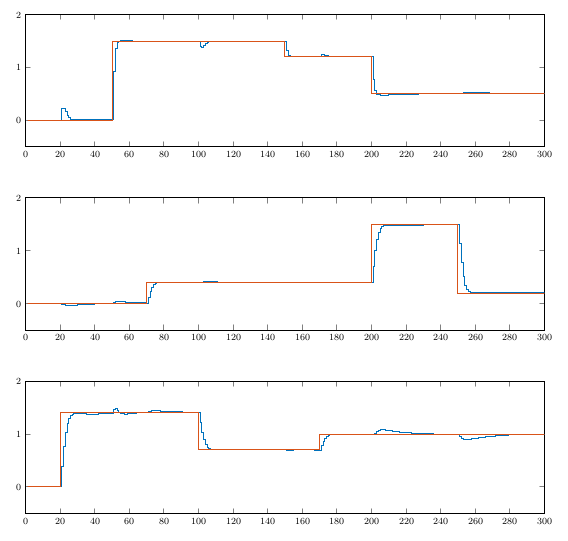
\includegraphics[scale=0.4]{images/innydmc.png} %%do poprawy jak już będą ładne
          			 \caption{Wyniki wielowymiarowej regulacji z zastosowaniem algorytmu GPC}
		\end{figure}
	\end{center}
\end{frame}
